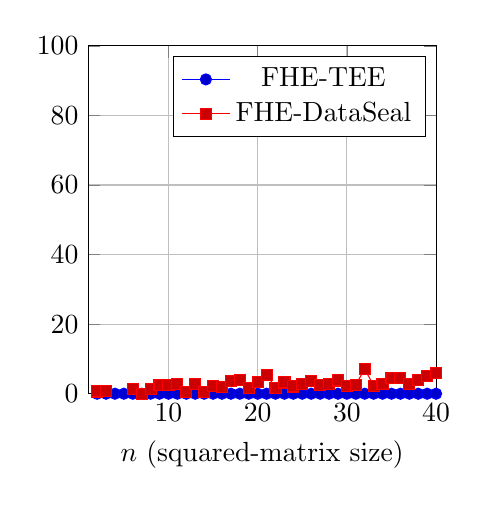
\begin{tikzpicture}
\begin{axis}[
    width=6cm, % Set the width of the plot to the text width of the subfigure
    height=6cm, % You can adjust the height as needed
    xlabel={$n$ (squared-matrix size)},
    legend pos=north east,
    grid=both,
    xmin=1, xmax=40,
    ymin=0, ymax=100
]
\addplot table {
n	FHE-TEE
2	0
3	0
4	0
5	0
6	0
7	0
8	0
9	0
10	0
11	0
12	0
13	0
14	0
15	0
16	0
17	0
18	0
19	0
20	0
21	0
22	0
23	0
24	0
25	0
26	0
27	0
28	0
29	0
30	0
31	0
32	0
33	0
34	0
35	0
36	0
37	0
38	0
39	0
40	0
41	0
42	0
43	0
44	0
45	0
46	0
47	0
48	0
49	0
50	0
51	0
52	0
53	0
54	0
55	0
56	0
57	0
58	0
59	0
60	0
61	0
62	0
63	0
64	0
};
\addlegendentry{FHE-TEE}

\addplot table {
n	FHE-DataSeal
2	0.6454989532
3	0.7694087701
4	-0.4751131222
5	-1.028910138
6	1.338116388
7	0.03425830764
8	1.35979632
9	2.526046214
10	2.569903701
11	2.892848878
12	0.5324074074
13	2.853150111
14	0.6123627961
15	2.276176024
16	1.92563465
17	3.690490116
18	3.854439592
19	1.560693642
20	3.395169758
21	5.484693878
22	1.717089125
23	3.24170726
24	2.090247453
25	2.748278679
26	3.659874156
27	2.422830518
28	2.909451344
29	3.807017544
30	2.318266542
31	2.573058563
32	7.148297885
33	2.272198977
34	2.858136704
35	4.463714136
36	4.584377002
37	2.690349456
38	3.990678707
39	5.187319885
40	5.904716645
};
\addlegendentry{FHE-DataSeal}


\end{axis}
\end{tikzpicture}